\documentclass[12pt]{article}

\usepackage[utf8]{inputenc}
\usepackage[T1]{fontenc}
\usepackage[english]{babel}
\usepackage{amssymb}
\usepackage[export]{adjustbox} % allows to use extra argument in \includegraphics{imagefile}, e.g.: \includegraphics{imagefile, center}



\title{Report: Assignment 1: \\Big Data Analytics Programming}
\author{Andreas Hinderyckx}
\date{December 2021} 

\usepackage{graphicx}
\usepackage{xcolor}
\usepackage{caption}

\begin{document}

\newcommand{\todo}{\fbox{\textbf{\textcolor{red}{TODO}}} }
\newcommand{\sctf}[1]{10\mathrm{e}{-#1}}
\maketitle

\newpage

\section{Bugs}
\section{Learning Curves}
The learning curves for the Perceptron (PC) and Very Fast Decision Tree (VFDT) run on the \texttt{clean} datasets are shown in figures \ref{fig:pc_clean} and \ref{fig:vfdt_clean} respectively. What's remarkable is that the PC achieves almost perfect accuracy while the VFDT only achieves an accuracy of approximately $75\%$ on the clean data. The accuracy of the PC shows, however, much more oscillation whereas the VFDT's accuracy follows a more stable course. After around $100.000.000$ examples have been trained with, we can clearly see the change of model used to generate the data in both graphs: both the PC's and VFDT's accuracy take a steep drop to $55\%$ accuracy. The PC quickly recovers back up to its original state, wheras the VFDT doesn't reach the same accuracy it had before: this could be due to the VFDT being overfit to the previously used model to generate the data, whereas the PC's weights can be changed entirely as needed.	

Tested on the \texttt{noisy} data set, we acquire the learning curves shown in figures \ref{fig:pc_noise} and \ref{fig:vfdt_noise}. Now the oscillations of the PC's accuracy become clearly visible: it struggles to learn the model due to the added noise. The VFDT's graph is highly similar to its graph for the \texttt{clean} data, with a reduction of achieved accuracy of $10\%$ and some extra oscillation in the accuracy.


\begin{figure}
	\centering
	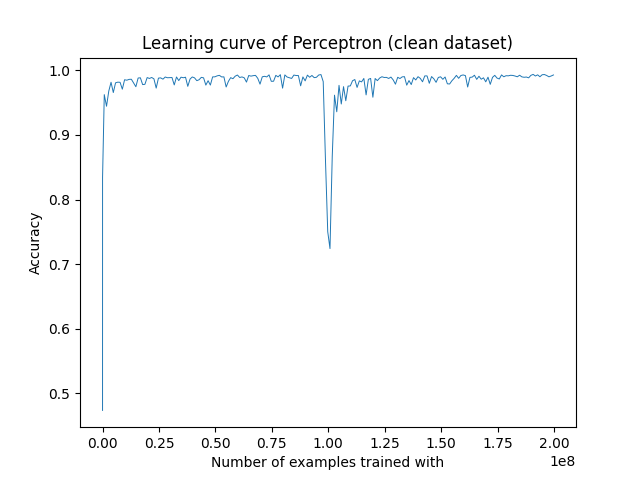
\includegraphics[width=.8\linewidth]{../plots/pc_clean}
	\caption{Learning curve of PC on the \texttt{clean} dataset}
	\label{fig:pc_clean}
\end{figure}
\begin{figure}
	\centering
	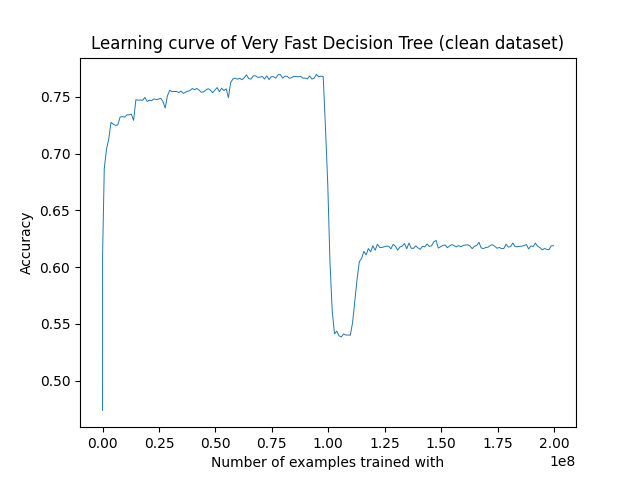
\includegraphics[width=.8\linewidth]{../plots/vfdt_clean}
	\caption{Learning curve of VFDT on the \texttt{clean} dataset}
	\label{fig:vfdt_clean}
\end{figure}
\begin{figure}
	\centering
	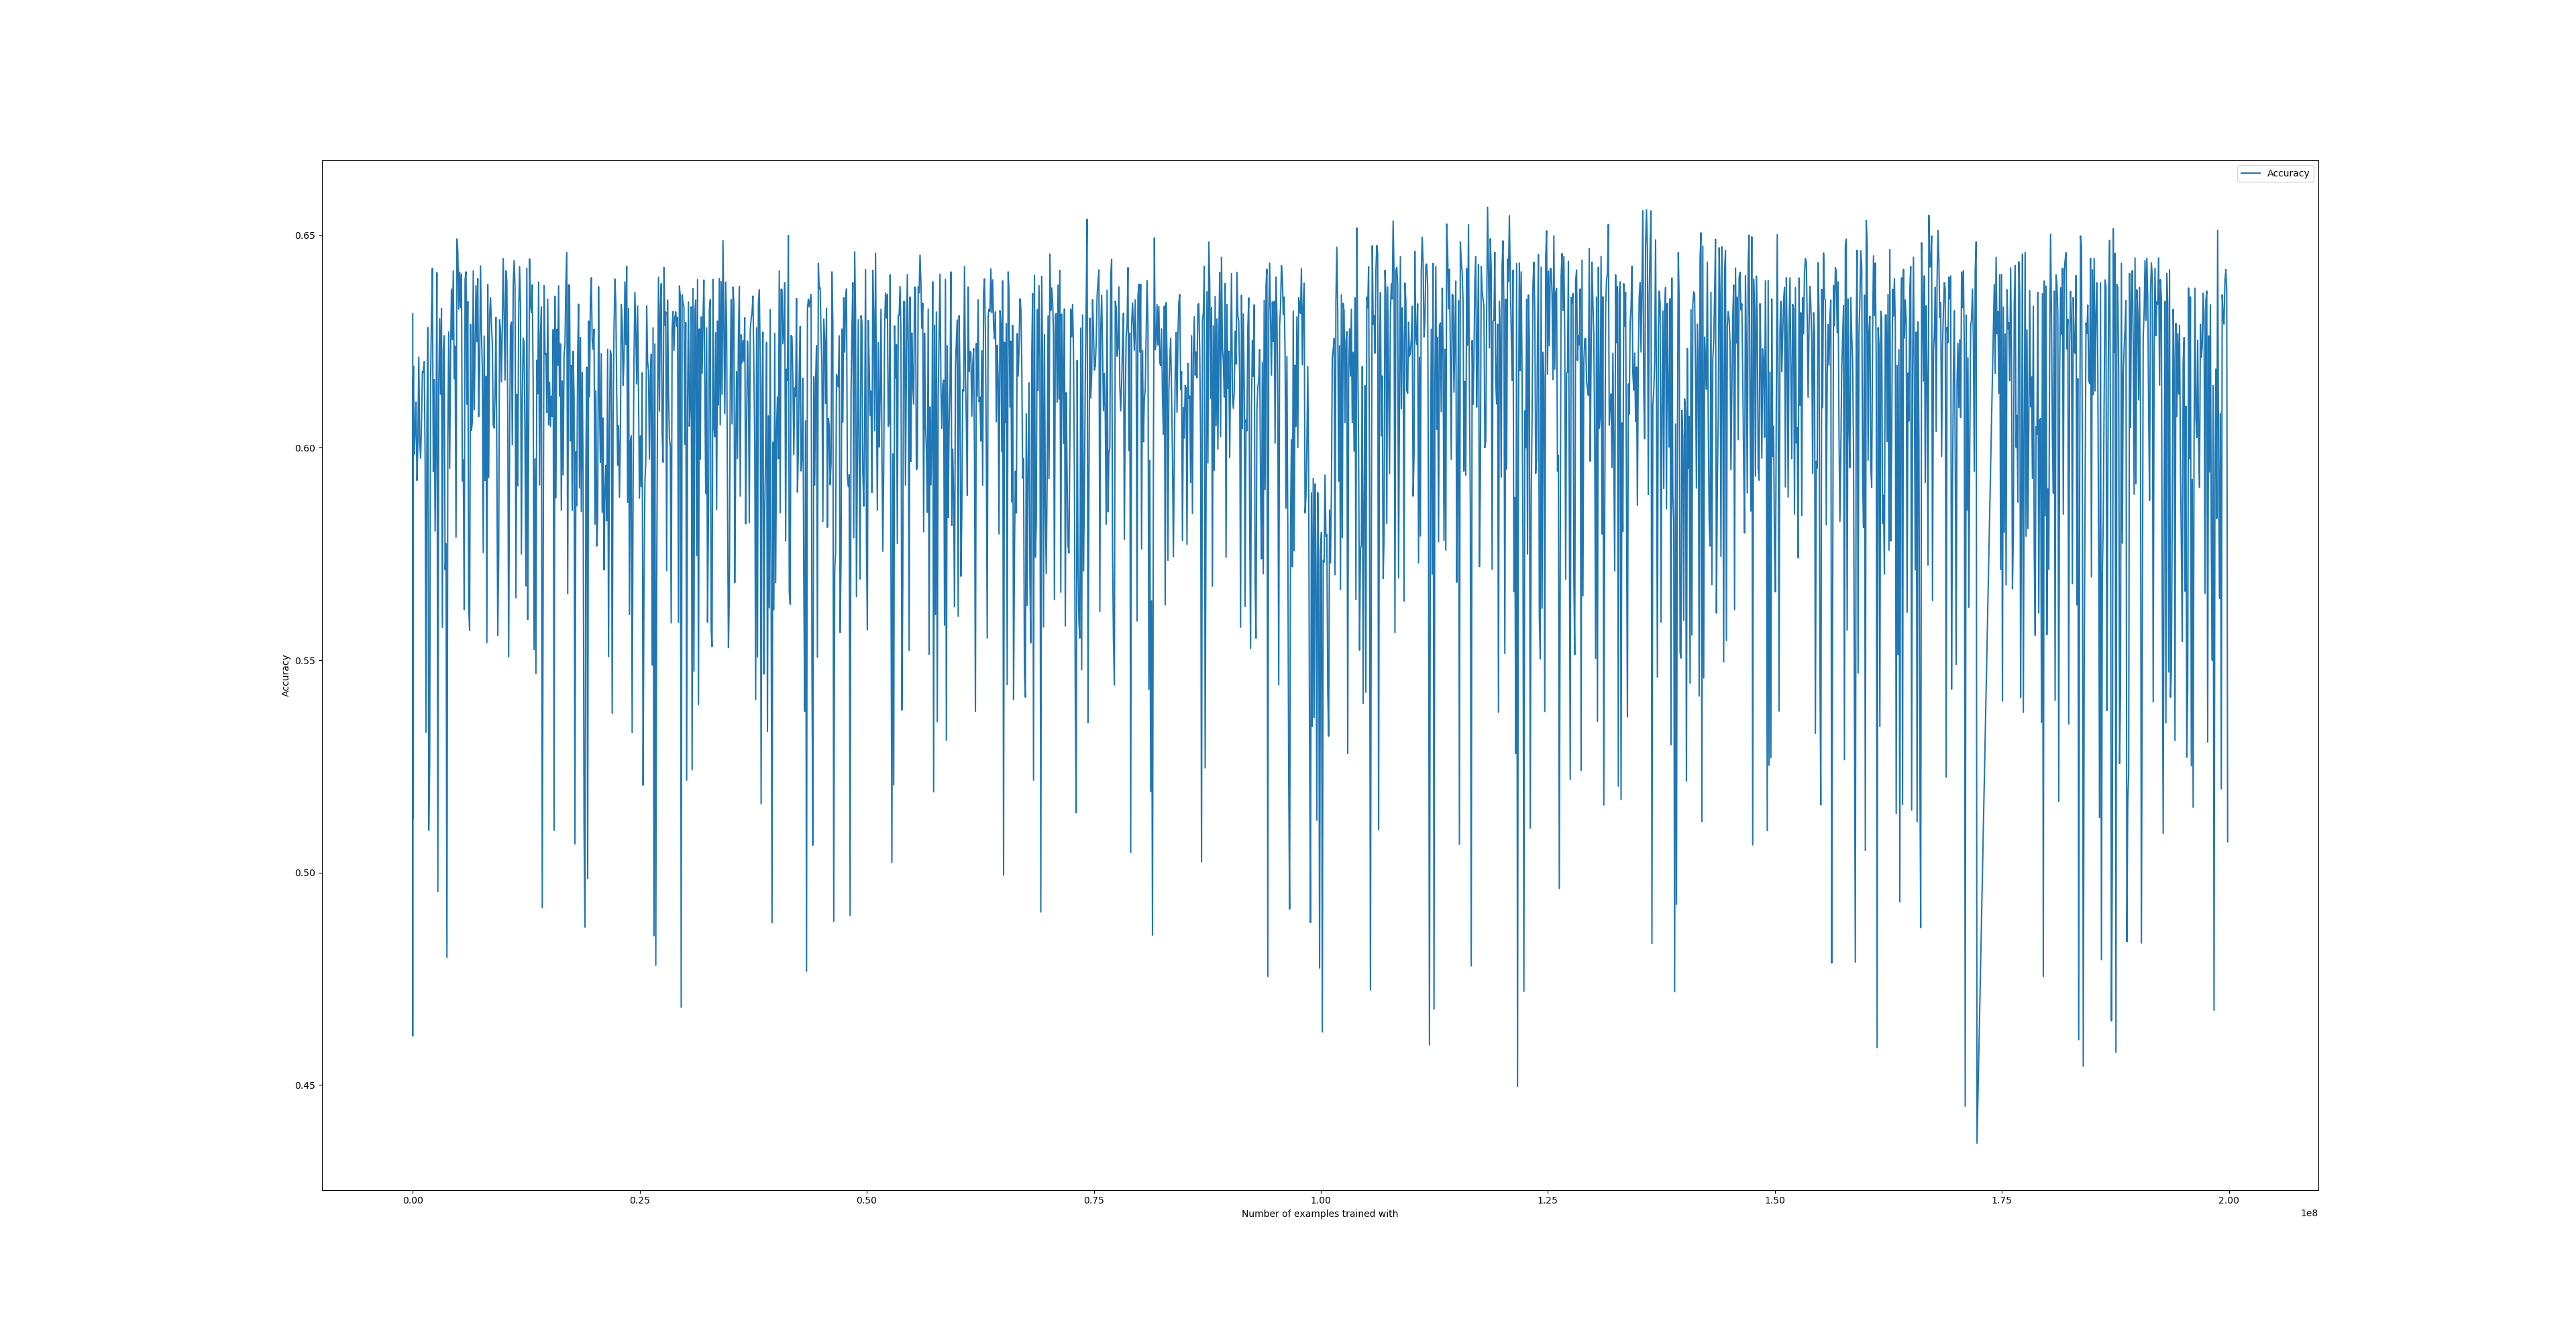
\includegraphics[width=.8\linewidth]{../plots/pc_noise}
	\caption{Learning curve of PC on the \texttt{noisy} dataset}
	\label{fig:pc_noise}
\end{figure}
\begin{figure}
	\centering
	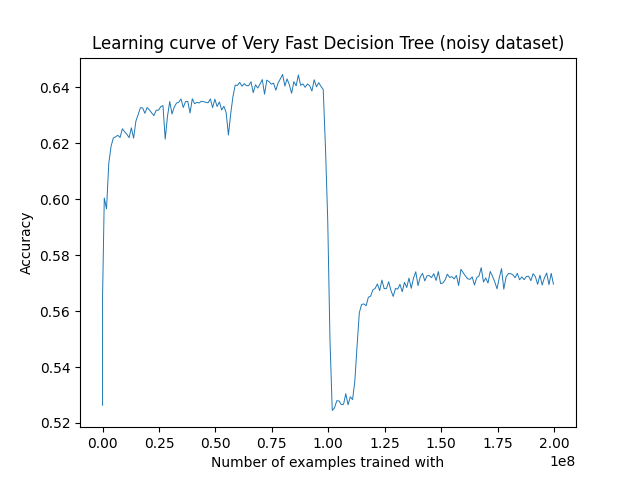
\includegraphics[width=.8\linewidth]{../plots/vfdt_noise}
	\caption{Learning curve of VFDT on the \texttt{noisy} dataset}
	\label{fig:vfdt_noise}
\end{figure}
\section{Experiments}
To study the effect of different parameters present in the programs, we pose the following questions:
\begin{enumerate}
	\item What's the effect of varying $\eta$ (eta) in the PC implementation?
	\item What's the effect of varying $\delta$ (delta) in the VFDT implementation?
	\item What's the effect of varying $\tau$ (tau) in the VFDT implementation?
	\item What's the effect of varying $n_{min}$ (how often split function is recalculated) in the VFDT implementation?
\end{enumerate}

The learning curves for the PC with varying values for $\eta$ on the \texttt{clean} data set are shown in figure \ref{fig:pc_etas}. We notice that smaller learning learning rates result in  less oscillating accuracies throughout the learning process. 

For studying the parameters of the VFDT, we use the \texttt{clean} dataset. In figure \ref{fig:vfdt_deltas} we can see that varying $\delta$ affects the speed at which accuracy is gained. In the initial learning phase $\delta := \sctf{9}$ seems to gain accuracy the quickest, while after the concept drift $\delta := \sctf{7}$ is more succesful (see fig. \ref{fig:vfdt_delta_zoom}). In general, small values for $\delta$ lead to higher accuracy: this is what we expect, as increasing $\delta$ increases the Hoeffding bound and thus will wait for a higher difference between the two highest split evaluation values before splitting. From figure \ref{fig:vfdt_taus} we can deduce that smaller values of $\tau$ increase the learning efficiency: this makes sense as the algorithm spends less time on deciding between minor differences in split evaluations and will be able to split sooner on these cases. We also note that for larger values of $\tau$, the experiments didn't finish due to excessive memory usage, as the algorithm will then split more often and thus consume more memory as $\tau$ increases. Finally, increasing $n_{min}$ implies the VFDT will re-compute the split evaluation function less frequently, which could increase the computation times, but should decrease the rate at which is learned, as valid splits are discovered with a delay. These assumptions are confirmed by figure \ref{fig:vfdt_nmins}, of which an enlarged view can be seen in figure \ref{fig:vfdt_nmins_zoom}.

\begin{figure}
	
	\centering
	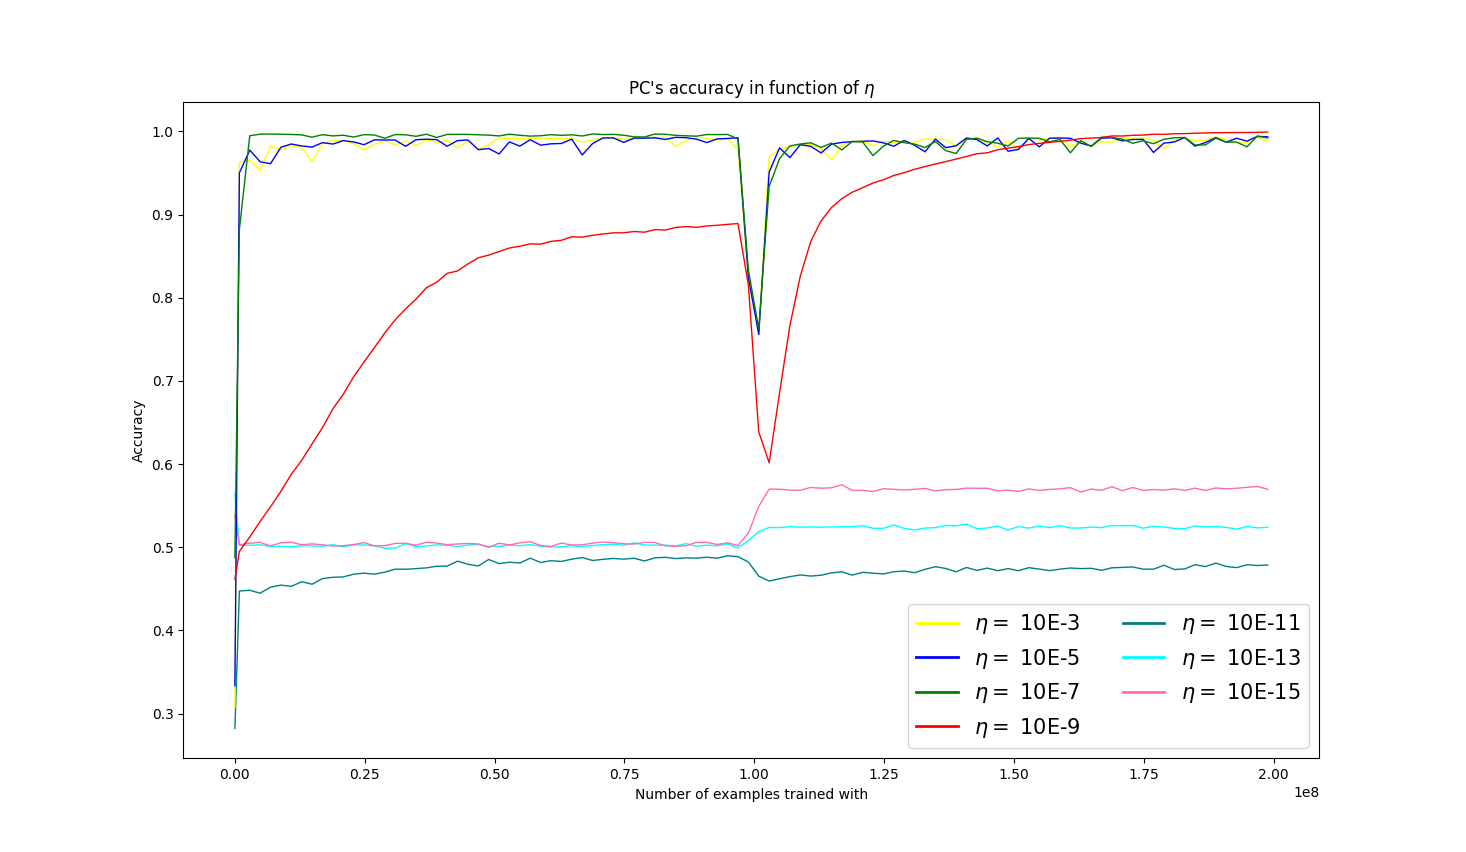
\includegraphics[width=1.6\linewidth, center]{./img/pc_etas.png}
	\caption{Effect of varying $\eta$}
	\label{fig:pc_etas}	
\end{figure}
\begin{figure}
	\centering
	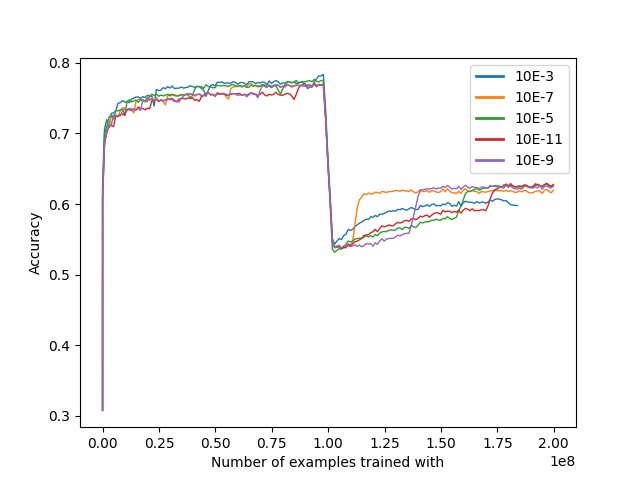
\includegraphics[width=.8\linewidth]{./img/vfdt_deltas.png}
	\caption{Effect of varying $\delta$}
	\label{fig:vfdt_deltas}	
\end{figure}
\begin{figure}
	\centering
	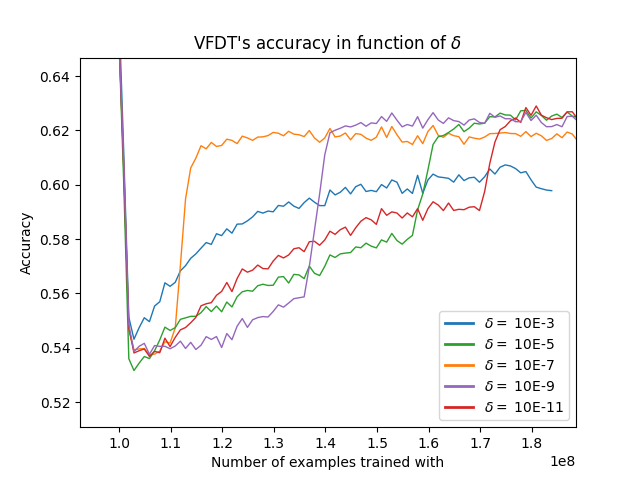
\includegraphics[width=.8\linewidth]{./img/vfdt_delta_zoom.png}
	\caption{Enlarged view of figure \ref{fig:vfdt_deltas}}
	\label{fig:vfdt_delta_zoom}	
\end{figure}
\begin{figure}
	\centering
	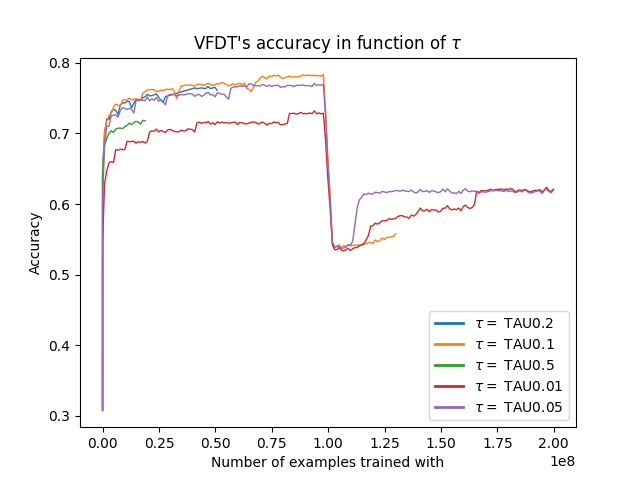
\includegraphics[width=.8\linewidth]{./img/vfdt_taus.png}
	\caption{Effect of varying $\tau$}
	\label{fig:vfdt_taus}	
\end{figure}
\begin{figure}
	\centering
	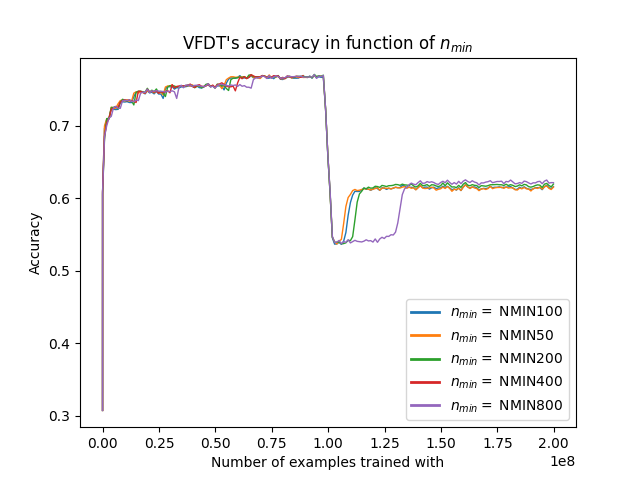
\includegraphics[width=.8\linewidth]{./img/vfdt_nmin.png}
	\caption{Effect of varying $n_{min}$}
	\label{fig:vfdt_nmins}	
\end{figure}
\begin{figure}
	\centering
	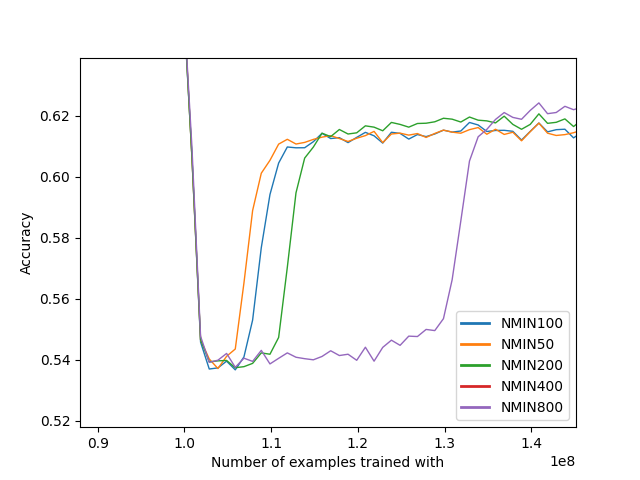
\includegraphics[width=.8\linewidth]{../code/experiments/vfdt/plots/vfdt_nmin_zoom.png}
	\caption{Enlarged view of figure \ref{fig:vfdt_nmins}}
	\label{fig:vfdt_nmins_zoom}	
\end{figure}


\end{document}
